\documentclass[tikz,border=3pt]{standalone}
\usepackage[utf8]{inputenc}
\usepackage[T1]{fontenc}
\usepackage{lmodern}
\renewcommand{\familydefault}{\sfdefault}
\usepackage{sansmath}\sansmath
\usepackage{chemfig}
\usepackage{pgfplots}\pgfplotsset{compat=1.18,/pgf/number format/use comma,/pgf/number format/1000 sep={.}}
\usetikzlibrary{arrows.meta,calc,positioning,decorations.pathmorphing,patterns}
% paleta del sitio
\definecolor{nar}{HTML}{E8680C}\definecolor{narc}{HTML}{FFB35C}\definecolor{hielo}{HTML}{FFF3E8}
\definecolor{tinta}{HTML}{1D1D1F}\definecolor{gris}{HTML}{6E6E73}\definecolor{lila}{HTML}{7C5CF0}
\definecolor{azul}{HTML}{2F6FD6}\definecolor{menta}{HTML}{17A673}\definecolor{coral}{HTML}{E8342A}
\tikzset{cel/.style={draw=gris,fill=hielo,line width=0.9pt},nuc/.style={draw=gris!70,line width=0.6pt},
fib/.style={gris!55,line width=0.35pt},eti/.style={font=\footnotesize,text=tinta,align=center},
num/.style={circle,draw=nar,fill=white,text=nar,font=\small\bfseries,inner sep=1.2pt,minimum size=13pt},
fl/.style={-{Stealth[length=2.6mm]},gris,line width=0.9pt}}
\begin{document}
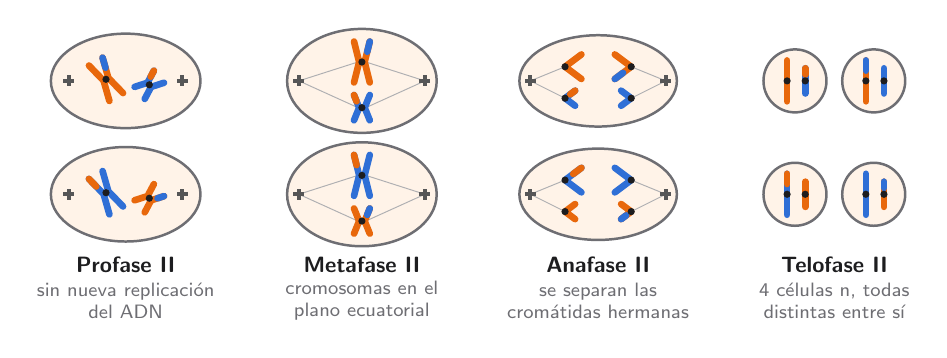
\begin{tikzpicture}[font=\small]
\draw[cel] (0,0.72) ellipse (0.95 and 0.6);
\begin{scope}[shift={(-0.25,0.74)},rotate=30]\draw[nar,line width=2.4pt,line cap=round,line join=round] (-0.1,0.26)--(-0.035,0)--(-0.1,-0.26);\end{scope}
\begin{scope}[shift={(-0.25,0.74)},rotate=30]\draw[nar,line width=2.4pt,line cap=round,line join=round] (0.1,0.26)--(0.035,0)--(0.1,-0.26);\draw[azul,line width=2.4pt,line cap=round] (0.1,0.26)--(0.068,0.13);\end{scope}
\fill[tinta] (-0.25,0.74) circle (1.3pt);
\begin{scope}[shift={(0.3,0.67)},rotate=-50]\draw[azul,line width=2.4pt,line cap=round,line join=round] (-0.1,0.16)--(-0.035,0)--(-0.1,-0.16);\draw[nar,line width=2.4pt,line cap=round] (-0.1,0.16)--(-0.068,0.08);\end{scope}
\begin{scope}[shift={(0.3,0.67)},rotate=-50]\draw[azul,line width=2.4pt,line cap=round,line join=round] (0.1,0.16)--(0.035,0)--(0.1,-0.16);\end{scope}
\fill[tinta] (0.3,0.67) circle (1.3pt);
\fill[tinta!75] (-0.79,0.695) rectangle (-0.65,0.745);\fill[tinta!75] (-0.745,0.65) rectangle (-0.695,0.79);
\fill[tinta!75] (0.65,0.695) rectangle (0.79,0.745);\fill[tinta!75] (0.695,0.65) rectangle (0.745,0.79);
\draw[cel] (0,-0.72) ellipse (0.95 and 0.6);
\begin{scope}[shift={(-0.25,-0.7)},rotate=30]\draw[azul,line width=2.4pt,line cap=round,line join=round] (-0.1,0.26)--(-0.035,0)--(-0.1,-0.26);\draw[nar,line width=2.4pt,line cap=round] (-0.1,0.26)--(-0.068,0.13);\end{scope}
\begin{scope}[shift={(-0.25,-0.7)},rotate=30]\draw[azul,line width=2.4pt,line cap=round,line join=round] (0.1,0.26)--(0.035,0)--(0.1,-0.26);\end{scope}
\fill[tinta] (-0.25,-0.7) circle (1.3pt);
\begin{scope}[shift={(0.3,-0.77)},rotate=-50]\draw[nar,line width=2.4pt,line cap=round,line join=round] (-0.1,0.16)--(-0.035,0)--(-0.1,-0.16);\end{scope}
\begin{scope}[shift={(0.3,-0.77)},rotate=-50]\draw[nar,line width=2.4pt,line cap=round,line join=round] (0.1,0.16)--(0.035,0)--(0.1,-0.16);\draw[azul,line width=2.4pt,line cap=round] (0.1,0.16)--(0.068,0.08);\end{scope}
\fill[tinta] (0.3,-0.77) circle (1.3pt);
\fill[tinta!75] (-0.79,-0.745) rectangle (-0.65,-0.695);\fill[tinta!75] (-0.745,-0.79) rectangle (-0.695,-0.65);
\fill[tinta!75] (0.65,-0.745) rectangle (0.79,-0.695);\fill[tinta!75] (0.695,-0.79) rectangle (0.745,-0.65);
\draw[cel] (3,0.72) ellipse (0.95 and 0.66);
\draw[fib] (2.2,0.72)--(2.95,0.96);
\draw[fib] (3.8,0.72)--(3.05,0.96);
\draw[fib] (2.2,0.72)--(2.95,0.38);
\draw[fib] (3.8,0.72)--(3.05,0.38);
\begin{scope}[shift={(3,0.96)},rotate=0]\draw[nar,line width=2.4pt,line cap=round,line join=round] (-0.1,0.26)--(-0.035,0)--(-0.1,-0.26);\end{scope}
\begin{scope}[shift={(3,0.96)},rotate=0]\draw[nar,line width=2.4pt,line cap=round,line join=round] (0.1,0.26)--(0.035,0)--(0.1,-0.26);\draw[azul,line width=2.4pt,line cap=round] (0.1,0.26)--(0.068,0.13);\end{scope}
\fill[tinta] (3,0.96) circle (1.3pt);
\begin{scope}[shift={(3,0.38)},rotate=0]\draw[azul,line width=2.4pt,line cap=round,line join=round] (-0.1,0.16)--(-0.035,0)--(-0.1,-0.16);\draw[nar,line width=2.4pt,line cap=round] (-0.1,0.16)--(-0.068,0.08);\end{scope}
\begin{scope}[shift={(3,0.38)},rotate=0]\draw[azul,line width=2.4pt,line cap=round,line join=round] (0.1,0.16)--(0.035,0)--(0.1,-0.16);\end{scope}
\fill[tinta] (3,0.38) circle (1.3pt);
\fill[tinta!75] (2.13,0.695) rectangle (2.27,0.745);\fill[tinta!75] (2.175,0.65) rectangle (2.225,0.79);
\fill[tinta!75] (3.73,0.695) rectangle (3.87,0.745);\fill[tinta!75] (3.775,0.65) rectangle (3.825,0.79);
\draw[cel] (3,-0.72) ellipse (0.95 and 0.66);
\draw[fib] (2.2,-0.72)--(2.95,-0.48);
\draw[fib] (3.8,-0.72)--(3.05,-0.48);
\draw[fib] (2.2,-0.72)--(2.95,-1.06);
\draw[fib] (3.8,-0.72)--(3.05,-1.06);
\begin{scope}[shift={(3,-0.48)},rotate=0]\draw[azul,line width=2.4pt,line cap=round,line join=round] (-0.1,0.26)--(-0.035,0)--(-0.1,-0.26);\draw[nar,line width=2.4pt,line cap=round] (-0.1,0.26)--(-0.068,0.13);\end{scope}
\begin{scope}[shift={(3,-0.48)},rotate=0]\draw[azul,line width=2.4pt,line cap=round,line join=round] (0.1,0.26)--(0.035,0)--(0.1,-0.26);\end{scope}
\fill[tinta] (3,-0.48) circle (1.3pt);
\begin{scope}[shift={(3,-1.06)},rotate=0]\draw[nar,line width=2.4pt,line cap=round,line join=round] (-0.1,0.16)--(-0.035,0)--(-0.1,-0.16);\end{scope}
\begin{scope}[shift={(3,-1.06)},rotate=0]\draw[nar,line width=2.4pt,line cap=round,line join=round] (0.1,0.16)--(0.035,0)--(0.1,-0.16);\draw[azul,line width=2.4pt,line cap=round] (0.1,0.16)--(0.068,0.08);\end{scope}
\fill[tinta] (3,-1.06) circle (1.3pt);
\fill[tinta!75] (2.13,-0.745) rectangle (2.27,-0.695);\fill[tinta!75] (2.175,-0.79) rectangle (2.225,-0.65);
\fill[tinta!75] (3.73,-0.745) rectangle (3.87,-0.695);\fill[tinta!75] (3.775,-0.79) rectangle (3.825,-0.65);
\draw[cel] (6,0.72) ellipse (1 and 0.58);
\draw[fib] (5.14,0.72)--(5.58,0.9);
\draw[fib] (6.86,0.72)--(6.42,0.9);
\draw[fib] (5.14,0.72)--(5.58,0.5);
\draw[fib] (6.86,0.72)--(6.42,0.5);
\begin{scope}[shift={(5.58,0.9)},rotate=90]\draw[nar,line width=2.4pt,line cap=round,line join=round] (-0.156,-0.208)--(0,0)--(0.156,-0.208);\end{scope}
\fill[tinta] (5.58,0.9) circle (1.3pt);
\begin{scope}[shift={(6.42,0.9)},rotate=-90]\draw[nar,line width=2.4pt,line cap=round,line join=round] (-0.156,-0.208)--(0,0)--(0.156,-0.208);\draw[azul,line width=2.4pt,line cap=round] (0.156,-0.208)--(0.078,-0.104);\end{scope}
\fill[tinta] (6.42,0.9) circle (1.3pt);
\begin{scope}[shift={(5.58,0.5)},rotate=90]\draw[azul,line width=2.4pt,line cap=round,line join=round] (-0.096,-0.128)--(0,0)--(0.096,-0.128);\draw[nar,line width=2.4pt,line cap=round] (0.096,-0.128)--(0.048,-0.064);\end{scope}
\fill[tinta] (5.58,0.5) circle (1.3pt);
\begin{scope}[shift={(6.42,0.5)},rotate=-90]\draw[azul,line width=2.4pt,line cap=round,line join=round] (-0.096,-0.128)--(0,0)--(0.096,-0.128);\end{scope}
\fill[tinta] (6.42,0.5) circle (1.3pt);
\fill[tinta!75] (5.07,0.695) rectangle (5.21,0.745);\fill[tinta!75] (5.115,0.65) rectangle (5.165,0.79);
\fill[tinta!75] (6.79,0.695) rectangle (6.93,0.745);\fill[tinta!75] (6.835,0.65) rectangle (6.885,0.79);
\draw[cel] (6,-0.72) ellipse (1 and 0.58);
\draw[fib] (5.14,-0.72)--(5.58,-0.54);
\draw[fib] (6.86,-0.72)--(6.42,-0.54);
\draw[fib] (5.14,-0.72)--(5.58,-0.94);
\draw[fib] (6.86,-0.72)--(6.42,-0.94);
\begin{scope}[shift={(5.58,-0.54)},rotate=90]\draw[azul,line width=2.4pt,line cap=round,line join=round] (-0.156,-0.208)--(0,0)--(0.156,-0.208);\draw[nar,line width=2.4pt,line cap=round] (0.156,-0.208)--(0.078,-0.104);\end{scope}
\fill[tinta] (5.58,-0.54) circle (1.3pt);
\begin{scope}[shift={(6.42,-0.54)},rotate=-90]\draw[azul,line width=2.4pt,line cap=round,line join=round] (-0.156,-0.208)--(0,0)--(0.156,-0.208);\end{scope}
\fill[tinta] (6.42,-0.54) circle (1.3pt);
\begin{scope}[shift={(5.58,-0.94)},rotate=90]\draw[nar,line width=2.4pt,line cap=round,line join=round] (-0.096,-0.128)--(0,0)--(0.096,-0.128);\end{scope}
\fill[tinta] (5.58,-0.94) circle (1.3pt);
\begin{scope}[shift={(6.42,-0.94)},rotate=-90]\draw[nar,line width=2.4pt,line cap=round,line join=round] (-0.096,-0.128)--(0,0)--(0.096,-0.128);\draw[azul,line width=2.4pt,line cap=round] (0.096,-0.128)--(0.048,-0.064);\end{scope}
\fill[tinta] (6.42,-0.94) circle (1.3pt);
\fill[tinta!75] (5.07,-0.745) rectangle (5.21,-0.695);\fill[tinta!75] (5.115,-0.79) rectangle (5.165,-0.65);
\fill[tinta!75] (6.79,-0.745) rectangle (6.93,-0.695);\fill[tinta!75] (6.835,-0.79) rectangle (6.885,-0.65);
\draw[cel] (8.5,0.72) circle (0.4);
\begin{scope}[shift={(8.4,0.72)},rotate=0]\draw[nar,line width=2.4pt,line cap=round,line join=round] (0,0.26)--(0,0)--(0,-0.26);\end{scope}
\fill[tinta] (8.4,0.72) circle (1.3pt);
\begin{scope}[shift={(8.63,0.72)},rotate=0]\draw[azul,line width=2.4pt,line cap=round,line join=round] (0,0.16)--(0,0)--(0,-0.16);\draw[nar,line width=2.4pt,line cap=round] (0,0.16)--(0,0.08);\end{scope}
\fill[tinta] (8.63,0.72) circle (1.3pt);
\draw[cel] (9.5,0.72) circle (0.4);
\begin{scope}[shift={(9.4,0.72)},rotate=0]\draw[nar,line width=2.4pt,line cap=round,line join=round] (0,0.26)--(0,0)--(0,-0.26);\draw[azul,line width=2.4pt,line cap=round] (0,0.26)--(0,0.13);\end{scope}
\fill[tinta] (9.4,0.72) circle (1.3pt);
\begin{scope}[shift={(9.63,0.72)},rotate=0]\draw[azul,line width=2.4pt,line cap=round,line join=round] (0,0.16)--(0,0)--(0,-0.16);\end{scope}
\fill[tinta] (9.63,0.72) circle (1.3pt);
\draw[cel] (8.5,-0.72) circle (0.4);
\begin{scope}[shift={(8.4,-0.72)},rotate=0]\draw[azul,line width=2.4pt,line cap=round,line join=round] (0,0.26)--(0,0)--(0,-0.26);\draw[nar,line width=2.4pt,line cap=round] (0,0.26)--(0,0.13);\end{scope}
\fill[tinta] (8.4,-0.72) circle (1.3pt);
\begin{scope}[shift={(8.63,-0.72)},rotate=0]\draw[nar,line width=2.4pt,line cap=round,line join=round] (0,0.16)--(0,0)--(0,-0.16);\end{scope}
\fill[tinta] (8.63,-0.72) circle (1.3pt);
\draw[cel] (9.5,-0.72) circle (0.4);
\begin{scope}[shift={(9.4,-0.72)},rotate=0]\draw[azul,line width=2.4pt,line cap=round,line join=round] (0,0.26)--(0,0)--(0,-0.26);\end{scope}
\fill[tinta] (9.4,-0.72) circle (1.3pt);
\begin{scope}[shift={(9.63,-0.72)},rotate=0]\draw[nar,line width=2.4pt,line cap=round,line join=round] (0,0.16)--(0,0)--(0,-0.16);\draw[azul,line width=2.4pt,line cap=round] (0,0.16)--(0,0.08);\end{scope}
\fill[tinta] (9.63,-0.72) circle (1.3pt);
\node[eti] at (0,-1.62) {\textbf{Profase II}};
\node[eti,font=\scriptsize,text=gris] at (0,-2.07) {sin nueva replicación\\del ADN};
\node[eti] at (3,-1.62) {\textbf{Metafase II}};
\node[eti,font=\scriptsize,text=gris] at (3,-2.07) {cromosomas en el\\plano ecuatorial};
\node[eti] at (6,-1.62) {\textbf{Anafase II}};
\node[eti,font=\scriptsize,text=gris] at (6,-2.07) {se separan las\\cromátidas hermanas};
\node[eti] at (9,-1.62) {\textbf{Telofase II}};
\node[eti,font=\scriptsize,text=gris] at (9,-2.07) {4 células n, todas\\distintas entre sí};
\end{tikzpicture}
\end{document}
